\chapter{RESULTADOS E DISCUSSÃO}

Os resultados apresentados neste capítulo foram obtidos a partir da execução
real do software desenvolvido (\texttt{poetry run dashboard}), com as quatro
planilhas de origem carregadas e a análise processada. As figuras referenciadas
encontram-se no diretório \texttt{imagens/}.

\section{Configuração da análise}

A Tabela~\ref{tab:insumos} relaciona os insumos utilizados na análise. O sistema
consolida o inventário e a criticidade dos equipamentos com as ordens de serviço
(OS) provenientes de dois formatos distintos de planilha: o formato antigo e o
formato atual.

\begin{table}[H]
    \centering
    \captionsource{tab:insumos}{Insumos utilizados na análise}{Elaborado pelo autor (2026)}
    \begin{tabular}{ll}
        \hline
        \textbf{Insumo} & \textbf{Arquivo} \\
        \hline
        Inventário de equipamentos & \texttt{Inventario\_HC\_UFPE.csv} \\
        Criticidade & \texttt{planilha de equipamentos final.csv} \\
        OS --- formato antigo & \texttt{Corretivas\_Externas\_2018\_a\_2024.csv} \\
        OS --- formato atual & \texttt{ServicoExternoPeriodo20251113092221.csv} \\
        \hline
    \end{tabular}
\end{table}

A base processada compreende:

\begin{itemize}
    \item \textbf{Inventário total processado:} 2.511 equipamentos.
    \item \textbf{Ordens de serviço consolidadas (base bruta):} 2.883 OS
    (2.568 do formato antigo e 318 do atual).
    \item \textbf{Recorte de análise (filtro de setores críticos --- padrão do
    sistema):} 8 sub-setores de UTI Adulto, UTI Neonatal, Bloco Cirúrgico e
    Centro Obstétrico, totalizando 516 equipamentos.
\end{itemize}

Todos os indicadores a seguir referem-se ao recorte de 516 equipamentos dos
setores críticos.

\section{Indicadores principais (KPIs)}

A Tabela~\ref{tab:kpis} sintetiza os principais indicadores de desempenho do
recorte analisado.

\begin{table}[H]
    \centering
    \captionsource{tab:kpis}{Indicadores principais (KPIs) dos setores críticos}{Elaborado pelo autor (2026)}
    \begin{tabular}{lr}
        \hline
        \textbf{Indicador} & \textbf{Valor} \\
        \hline
        Total de equipamentos (setores críticos) & 516 \\
        Total de OS emitidas & 245 \\
        Gasto total em OS & R\$~315.613,59 \\
        Custo médio por OS & $\approx$ R\$~1.288 \\
        Idade média do parque & 7,3 anos \\
        Equipamentos com $\geq$ 10 anos & 97 (18,8\%) \\
        \hline
    \end{tabular}
\end{table}

Quanto à composição por criticidade, o recorte distribui-se em: Alta (3) = 134
equipamentos; Média (2) = 156; e Baixa (1) = 226. Em relação ao status, 100\%
constam como ``Em uso'', uma vez que a base não traz equipamentos baixados ou
inoperantes nesse recorte. A Figura~\ref{fig:aba_analise} apresenta a aba de
análise do dashboard.

\begin{figure}[H]
    \centering
    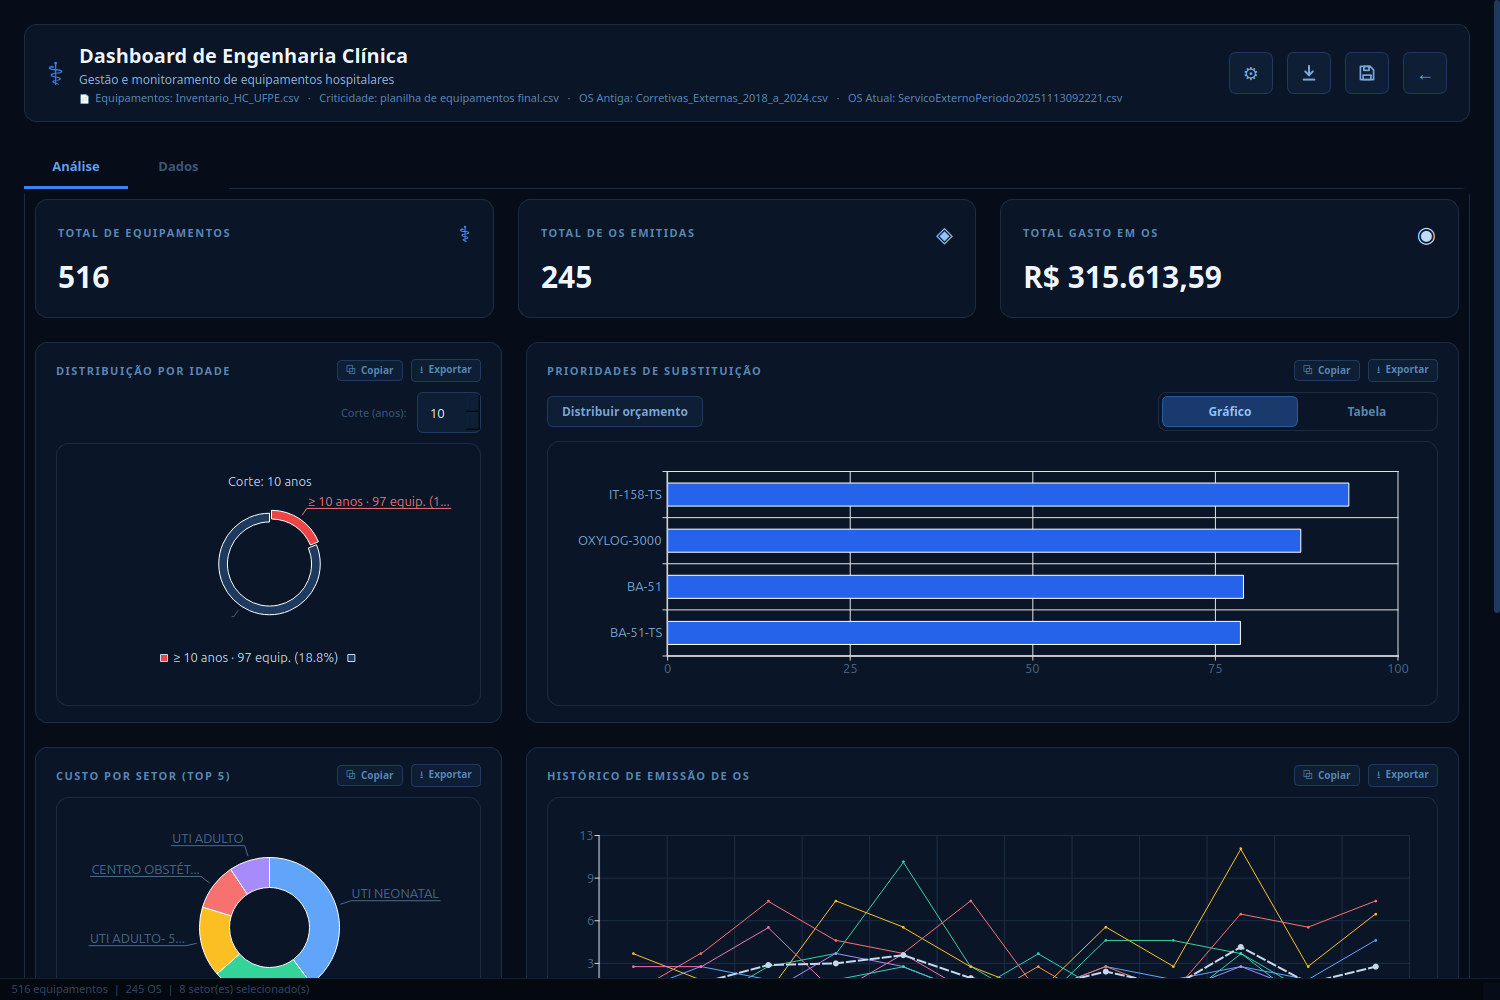
\includegraphics[width=\textwidth]{./imagens/01_aba_analise.png}
    \captionsource{fig:aba_analise}{Aba de análise do dashboard}{Elaborado pelo autor (2026)}
\end{figure}

\section{Distribuição por idade}

Dos 516 equipamentos, 97 (18,8\%) já ultrapassaram o corte de 10 anos de vida
útil. A idade média (7,3 anos) é puxada para baixo por aquisições recentes, mas
há uma cauda relevante de equipamentos antigos --- de até 23 anos ---, justamente
os de maior criticidade.

\section{Prioridade de substituição}

O \textit{score} (0--100) combina idade, criticidade e custo acumulado de
manutenção. A Tabela~\ref{tab:ranking} apresenta o topo do ranking de prioridade
de substituição.

\begin{table}[H]
    \centering
    \captionsource{tab:ranking}{Topo do ranking de prioridade de substituição}{Elaborado pelo autor (2026)}
    \begin{tabular}{clllccr}
        \hline
        \textbf{\#} & \textbf{Identificador} & \textbf{Modelo} & \textbf{Setor} & \textbf{Crit.} & \textbf{Idade} & \textbf{Score} \\
        \hline
        1 & HCPE-1311 & IT-158-TS & Centro Obstétrico & 3 & 23 & 100,0 \\
        2 & HCPE-0490 & OXYLOG-3000 & UTI Adulto & 3 & 17 & 93,3 \\
        3 & HCPE-1766 & BA-51 & Centro Obstétrico & 3 & 23 & 86,7 \\
        4 & HCPE-1220 & BA-51 & UTI Neonatal & 3 & 23 & 78,8 \\
        5 & HCPE-1256 & BA-51-TS & UTI Neonatal & 3 & 23 & 78,4 \\
        6 & HCPE-2667 & DX-3012 & UTI Adulto 5º & 3 & 14 & 74,9 \\
        7 & HCPE-0547 & BILITRON-3006-BTP & UTI Neonatal & 3 & 13 & 72,5 \\
        8 & HCPE-0549 & BILITRON-3006-BTP & UTI Neonatal & 3 & 13 & 72,2 \\
        \hline
    \end{tabular}
\end{table}

O topo do ranking é dominado por equipamentos de criticidade máxima (3) e idade
$\geq$ 13 anos, concentrados em UTI Neonatal e Centro Obstétrico (incubadoras e
aquecedores BA-51, fototerapia BILITRON, ventilador de transporte OXYLOG).

\section{Histórico de emissão de OS e custo por ano}

A Tabela~\ref{tab:historico} apresenta a evolução anual do número de OS, do custo
total e do custo médio por OS.

\begin{table}[H]
    \centering
    \captionsource{tab:historico}{Histórico de emissão de OS e custo por ano}{Elaborado pelo autor (2026)}
    \begin{tabular}{lrrr}
        \hline
        \textbf{Ano} & \textbf{OS} & \textbf{Custo total} & \textbf{Custo médio/OS} \\
        \hline
        2018 & 36 & R\$~47.377,68 & R\$~1.316 \\
        2019 & 23 & R\$~16.690,74 & R\$~726 \\
        2020 & 56 & R\$~30.341,51 & R\$~542 \\
        2021 & 56 & R\$~21.040,99 & R\$~376 \\
        2022 & 23 & R\$~6.431,00 & R\$~280 \\
        2023 & 21 & R\$~38.613,70 & R\$~1.839 \\
        2024 & 19 & R\$~76.557,06 & R\$~4.029 \\
        2025\textsuperscript{*} & 11 & R\$~78.560,91 & R\$~7.142 \\
        \hline
    \end{tabular}
\end{table}

\noindent \textsuperscript{*} 2025 é ano parcial (dados até 13/11/2025).

\begin{figure}[H]
    \centering
    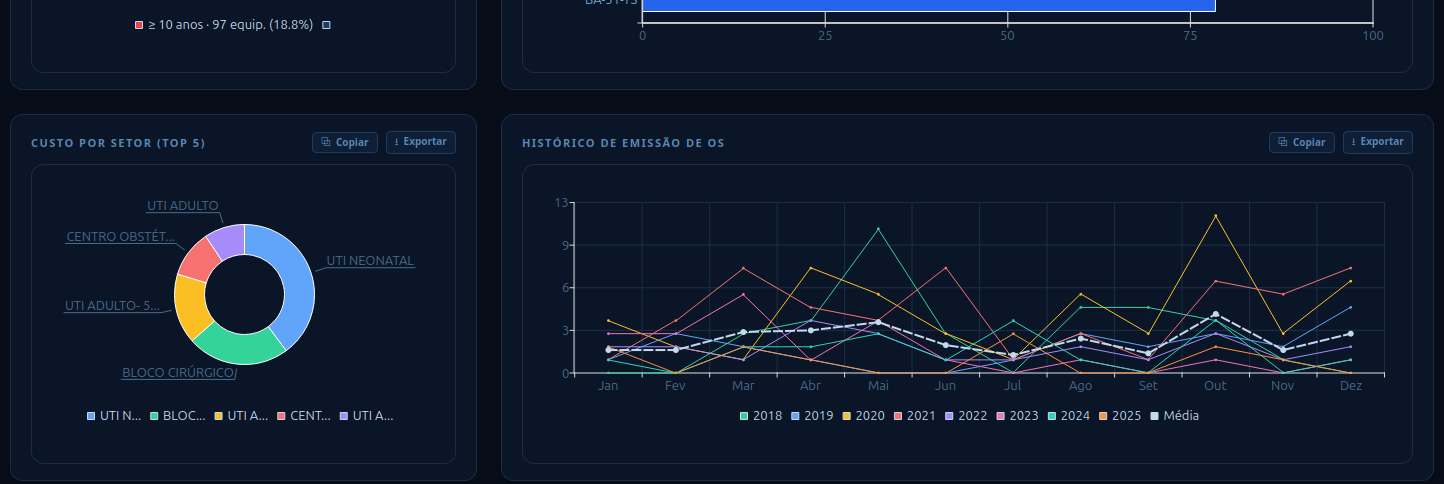
\includegraphics[width=\textwidth]{./imagens/02_custo_setor_historico_os.png}
    \captionsource{fig:custo_setor}{Custo por setor e histórico de OS}{Elaborado pelo autor (2026)}
\end{figure}

\begin{figure}[H]
    \centering
    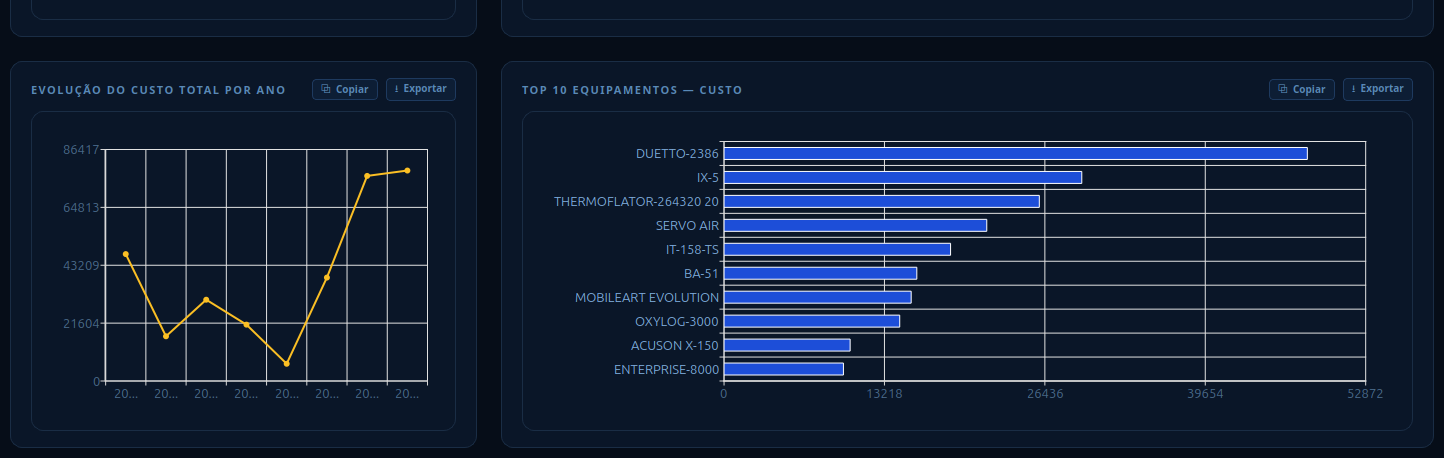
\includegraphics[width=\textwidth]{./imagens/03_evolucao_custo_top10.png}
    \captionsource{fig:evolucao_custo}{Evolução do custo e Top 10 equipamentos}{Elaborado pelo autor (2026)}
\end{figure}

\section{Concentração de custo por setor}

A Tabela~\ref{tab:custo_setor} evidencia a concentração do gasto corretivo por
setor.

\begin{table}[H]
    \centering
    \captionsource{tab:custo_setor}{Concentração de custo em OS por setor}{Elaborado pelo autor (2026)}
    \begin{tabular}{lrr}
        \hline
        \textbf{Setor} & \textbf{Custo em OS} & \textbf{Equip.} \\
        \hline
        UTI Neonatal & R\$~121.888,44 & 211 \\
        Bloco Cirúrgico & R\$~72.207,74 & 111 \\
        UTI Adulto 5º andar & R\$~49.639,32 & 61 \\
        Centro Obstétrico & R\$~33.444,51 & 91 \\
        UTI Adulto & R\$~28.595,79 & 24 \\
        UTI Adulto / URCC & R\$~9.837,79 & 1 \\
        \hline
    \end{tabular}
\end{table}

A UTI Neonatal, sozinha, responde por $\sim$39\% de todo o gasto corretivo do
recorte.

\section{Top 10 equipamentos por custo}

Agrupados por modelo, os dez equipamentos de maior custo são: DUETTO-2386 e IX-5
(incubadoras), THERMOFLATOR-264320 e SERVO AIR (ventilação), IT-158-TS, BA-51,
MOBILEART EVOLUTION, OXYLOG-3000, ACUSON X-150 e ENTERPRISE-8000. Predominam,
portanto, equipamentos de suporte à vida neonatal e de ventilação.

\section{Interpretação dos resultados}

\subsection{O custo de manutenção está migrando de ``muitas OS baratas'' para ``poucas OS caras''}

Entre 2020 e 2022, o parque gerava muitas ordens de baixo valor, com o custo
médio caindo até $\approx$ R\$~280/OS em 2022. A partir de 2023, o padrão se
inverte: o número de OS cai (de 56 para cerca de 11--21 por ano), mas o custo
médio por OS dispara --- de R\$~280 (2022) para R\$~4.029 (2024) e R\$~7.142
(2025). Esse é o comportamento típico de um parque envelhecendo: falhas mais
graves, peças mais caras e intervenções de maior porte. Mesmo com 2025 ainda
parcial, o gasto anual já supera o de 2024.

\subsection{Risco e custo estão concentrados nos mesmos setores}

A UTI Neonatal lidera o gasto corretivo ($\sim$39\% do total) e também concentra
os equipamentos do topo do ranking de substituição (BA-51, BILITRON, IX-5). Não
se trata de dispersão: há um núcleo crítico onde criticidade alta, idade elevada
e custo de manutenção coincidem --- exatamente o alvo no qual a substituição traz
maior retorno em segurança do paciente e redução de custo.

\subsection{Há uma cauda de equipamentos no fim da vida útil}

18,8\% do parque crítico já passou de 10 anos, e o topo do ranking chega a 23
anos de uso em equipamentos de criticidade 3. São candidatos diretos a
substituição planejada --- o software materializa isso no \textit{score} e na
funcionalidade ``Distribuir orçamento''.

\subsection{Valor da ferramenta para a gestão}

O dashboard converte cerca de 2.900 OS, dispersas em dois formatos de planilha,
em indicadores acionáveis: prioriza substituições por evidência (idade +
criticidade + custo), localiza onde o dinheiro está sendo gasto (UTI Neonatal) e
expõe a tendência de custo crescente --- insumos diretos para justificar
investimento em renovação de parque na engenharia clínica do HC-UFPE.

\subsection{Limitações}

O ano de 2025 é parcial; todos os equipamentos constam como ``Em uso'' (a base
não registra baixas); e os valores refletem apenas manutenção corretiva externa
do recorte escolhido (UTI, Bloco Cirúrgico e Centro Obstétrico). Trocar as
planilhas de OS (por exemplo, incluindo corretivas internas) ou ampliar os
setores no menu de configurações altera os números --- o que reforça o caráter
exploratório da ferramenta.
